%!TEX program = xelatex

\documentclass[compress]{beamer}
%--------------------------------------------------------------------------
% Common packages
%--------------------------------------------------------------------------

\definecolor{links}{HTML}{663000}
\hypersetup{colorlinks,linkcolor=,urlcolor=links}

\usepackage[english]{babel}
\usepackage{pgfpages} % required for notes on second screen
\usepackage{graphicx}

\usepackage{multicol}

\usepackage{tabularx,ragged2e}
\usepackage{booktabs}

\setlength{\emergencystretch}{3em}  % prevent overfull lines
\providecommand{\tightlist}{%
  \setlength{\itemsep}{0pt}\setlength{\parskip}{0pt}}


\usetheme{hri}

% Display the navigation bullet even without subsections
\usepackage{remreset}% tiny package containing just the \@removefromreset command
\makeatletter
\@removefromreset{subsection}{section}
\makeatother
\setcounter{subsection}{1}


\newcommand{\source}[2]{{\tiny\it Source: \href{#1}{#2}}}

\newcommand{\colvec}[2][.8]{%
  \scalebox{#1}{%
    \renewcommand{\arraystretch}{.8}%
    $\begin{bmatrix}#2\end{bmatrix}$%
  }
}


\usepackage{tikz}
\usetikzlibrary{mindmap,backgrounds,positioning,quotes}

\graphicspath{{figs/part6/}}

\title{ROCO318 \newline Mobile and Humanoid Robots}
\subtitle{Part 4 -- Localisation and Planning}

\date{}
\author{Séverin Lemaignan}
\institute{Centre for Neural Systems and Robotics\\{\bf Plymouth University}}

\begin{document}

\licenseframe{github.com/severin-lemaignan/module-mobile-and-humanoid-robots}

\maketitle

\begin{frame}{Pose and navigation}

Pose maintenance

\begin{itemize}
\item \textbf{Pose} (= position and orientation) \textbf{maintenance} is
  keeping a precise as possible estimate of the robot's pose.
\end{itemize}

Getting from A to B.

\begin{itemize}
\item Different from inverse kinematics, where an efficient manner is
  computed to get a robot in a certain state (position and orientation).
  Inverse kinematics work on a small scale (\textless{} meter).
\item Planning and navigation work on a larger scale (room, building,
  roadmap, \ldots{}).
\end{itemize}

\end{frame}

\begin{frame}{Planning and navigation -- traditional approach}

Today's industrial robots can operate \textbf{without any intelligence} because
their environment is static and very structured.

In mobile robotics, cognition and reasoning is primarily of geometric
nature, such as picking a safe path or determining where to go next.

\begin{itemize}
\item already been largely explored in literature for cases in which
  complete information about the current situation and the environment
  exists (e.g.
  \href{http://en.wikipedia.org/wiki/Travelling_salesman_problem}{travelling
  sales man problem} or
  \href{http://en.wikipedia.org/wiki/Route_inspection_problem}{route
  inspection problem}).
\end{itemize}

\end{frame}

\begin{frame}{Kiva systems: Beacon based localisation}
    \begin{center}
        \url{http://www.youtube.com/watch?v=lWsMdN7HMuA}

        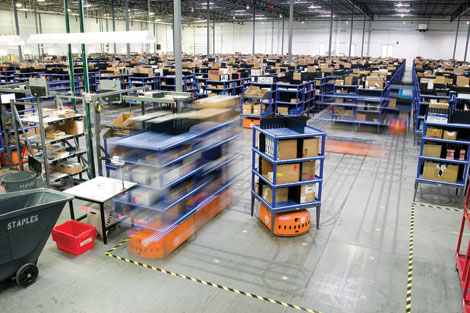
\includegraphics[width=0.8\linewidth]{kiva}
    \end{center}
\end{frame}

\section{Monte-Carlo Localisation}

\begin{frame}{Monte Carlo methods}

    \begin{columns}
        \begin{column}{0.5\linewidth}
            \textbf{Repeated random sampling to compute results}

            Used when it to difficult to calculate exact results:

            \begin{itemize}
                \item The system is too complex and calculating it through is too
                    computationally expensive
                \item There are too many variables and it is impossible to calculate all
                    posibilities
            \end{itemize}


        \end{column}
        \begin{column}{0.5\linewidth}
            \begin{center}
                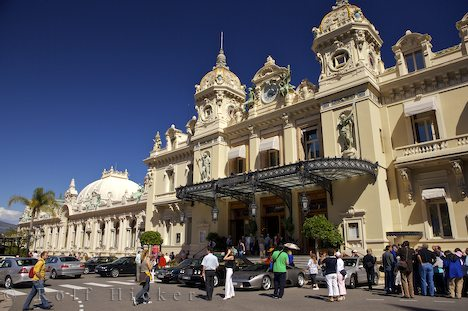
\includegraphics[width=\linewidth]{montecarlo}
            \end{center}

            \onslide<2>{
            Monte Carlo \emph{localisation} is MC methods applied to robot localisation.
            }
        \end{column}
    \end{columns}

\end{frame}

\imageframe{mcl_example}

\begin{frame}{Monte-Carlo Localisation -- Introduction}

\begin{itemize}
    \item Monte-Carlo Localisation (MCL) is a \href{http://en.wikipedia.org/wiki/Particle_filter}{particle
  filter}, which uses a set $S_t$ of $N$ particles at time
  $t$.
    \begin{align*}
        S_t &= \{s_t^i | i = 1\ldots N\} \\
        s^i &= \{l^i, p^i\} \text{ with } l^i = \{x^i, y^i, \theta^i\}
    \end{align*}
 \item<+-> For small maps, $N$ is in the hundreds, for larger maps you
  can have thousands of particles.
\item<+-> Each particle $s^i$ contains the pose of the particle and a posterior
    belief $p^i$.
\item<+-> The sum of all beliefs is 1: \[ \sum_{i=1}^N p^i = 1 \]
\end{itemize}

\end{frame}

\begin{frame}{Monte-Carlo Localisation -- Initialisation}

The $N$ particles are distributed on the map

\begin{itemize}
\item If the robot's position is not known, they are distributed randomly
    across the map with a probability $p=\frac{1}{N}$ (\emph{uniform
        distribution}).
\item If the robot's position is available, the initial particle
    distribution could be Gaussian around the robot (\emph{normal distribution}).
\end{itemize}

\pause 

Then , Monte Carlo Localisation runs through three steps:

\begin{enumerate}
\item Prediction phase (when the robot takes an action)
\item Update phase (when sensor data comes in)
\item Resampling phase
\end{enumerate}

\end{frame}

\begin{frame}{Monte-Carlo Localisation -- Prediction phase 1}

The robot performs an \textbf{action.} All $N$ particles are
    updated as follows:
    \Large
        \[ 
        \bubblemark{newp}p(s_t^i) = \sum_{j=1}^N
        p(l_t{}^j\bubblemark[0pt]{motionmodel}|l_{t-1}{}^i, a) \cdot p(s\bubblemark[0pt]{oldp}_{t-1}{}^i)
        \]
    \normalsize
    \begin{columns}
        \begin{column}{0.5\linewidth}
Example: repeated application of the prediction rule leads to gradual
  loss of pose accuracy.
        \end{column}
        \begin{column}{0.5\linewidth}
            \begin{center}
                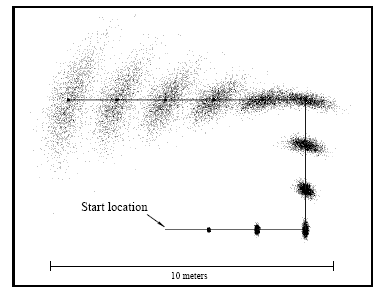
\includegraphics[width=\linewidth]{mcl_prediction}
            \end{center}
        \end{column}
    \end{columns}

    \bubble<1>[40][1][6.5cm]{motionmodel}{Motion model: what is the probability of ending up in the location of
particle $s_t$ after doing action $a$ at the location of
    particle $s_{t-1}$}

    \bubble<1>[130][0.5][3cm]{oldp}{Belief of $i^{th}$ particle at time $t-1$}

    \bubble<1>[0]{newp}{Updated belief of particle $i$}

\end{frame}

\begin{frame}{Monte-Carlo Loclaisation - Prediction phase 2}

The prediction phase \textbf{essentially moves all particles}.

Example: if the robot moves 10cm right and turn 10˚ counterclockwise, then all particles are
updated:
    \Large
    \[
        s_t^i = \{ \{ x_{t-1}^i + 0.1, y_{t-1}^i, \theta_{t-1}^i - 10^{\circ}\}, p\bubblemark[0pt]{oldnochange}_{t-1}^i\}
    \]
    \normalsize

\bubble<1>[90]{oldnochange}{Note, belief is not changed}
\pause

    This allows for a motion model to be implemented, by adding some noise.

    \only<2>{
    \large
    \begin{align*}
        s_t^1 &= \{ \{ x_{t-1}^1 + 0.11, y_{t-1}^1, \theta_{t-1}^1 - 10.3^{\circ}\}, p_{t-1}^1\} \\
        s_t^2 &= \{ \{ x_{t-1}^2 + 0.09, y_{t-1}^2, \theta_{t-1}^2 - 10.2^{\circ}\}, p_{t-1}^2\} \\
        ...
    \end{align*}
    \normalsize
    }

    \only<3>{
    This motion model should be based on the kinematics of your robot.
    \eg for a differential drive robot you would have a pretty accurate
    idea of how imprecise it is.
    }


\end{frame}

\begin{frame}{Monte-Carlo Localisation -- Update phase}

    \begin{itemize}
        \item The robot gets \textbf{new sensor data} in, all $N$ particles
            updated as follows:
            \Large
            \[ 
            p(s_t^i) = \bubblemark[0pt]{alpha}\alpha \cdot p(z_t\bubblemark[0pt]{sensormodel}|s_t^i) \cdot p(s_t^i)
            \]
            \normalsize
            \vspace{3em}
        \item The normalising constant $\alpha$ is calculated afterwards to make
            \[ \sum_{i=1}^N p^i = 1 \]
    \end{itemize}

    \bubble<1>[145][.8][4cm]{sensormodel}{Sensor model: what is the probability
    of seeing sensor reading $z_t$ at position $s_t$}

    \bubble<1>[40][.8][3cm]{alpha}{Normalisation constant: keeps to total $p$ value equal
    to 1}

\end{frame}

\begin{frame}{Monte-Carlo Localisation -- Resampling phase}

Generate a new set of particles by drawing randomly from the current
set. Likelihood is determined by $p$ values. Set the $p$ value
    of these new samples to $\frac{1}{N}$.

\begin{itemize}
\item You can think of drawing particles as a roulette wheel selection.
  Particles with a higher $p$ value have a higher chance of being
  selected into the new set. Also, a particle can be selected more than
  once
\end{itemize}

$p1$

$p2$

$p3$

$p4$

$p5$

$p7$

$p8$

$p9$

$p6$

\end{frame}

\begin{frame}{MCL -- Resamping phase (2)}

In addition, it is useful to add a small number of uniformly distributed
particles to the set of particles.

This helps the algorithm recover when it loses track of the robot's
position.

\begin{itemize}
\item This is know as thee ``kidnapped robot'' problem, and occurs when the
  robot loses track of its position, due to a malfunction or power
  outage.
\end{itemize}

\end{frame}

\begin{frame}[fragile]{Pseudocode (1)}

\begin{columns}
    \begin{column}{0.4\linewidth}
        
        \begin{pythoncode*}{frame=none,escapeinside=||}

# initialise all N particles
for i in range(1, N):
    S[i].x = random(x_max)
    S[i].y = random(y_max)
    S[i].|$\theta$| = random(2 * |$\pi$|)
    S[i].p = 1/N
\end{pythoncode*}
    \end{column}
    \begin{column}{0.6\linewidth}

\begin{pythoncode*}{frame=none,escapeinside=||}
while True:
    # prediction phase
    move_robot(x,y,theta)
    for i in range(1,N):
        move_particle(i, x, y, |$\theta$|)

    # update phase
    n = 0
    for i in range(1,N):
    TO BE FIXED
        S[i] = p(r||S[i].x, S[i].y, S[i].|$\theta$|) * S[i].p
        n = n + S[i].p

    # normalise
    for i in range(1,N):
        S[i].p = S[i].p/n

    # resample phase
    for i in range(1,M):
        draw_S1_with_high_S.p
        find_S2_with_lowest_S.p
        S2=S1
\end{pythoncode*}
    \end{column}
\end{columns}

\end{frame}

\begin{frame}{Pseudocode (2)}

\end{frame}

\begin{frame}{MCL -- Some properties}

Light on memory and computational resources.

\begin{itemize}
\item Markov Localisation uses much more memory, as it needs to keep track
  of belief at each location of the map even the ones that have a low
  belief. This also results in a computationally expensive algorithm.
\end{itemize}

``Any time'' algorithm: you can interrupt the algorithm and still get an
estimate out.

Powerful, yet efficient.

Easy to implement.

\end{frame}

\begin{frame}{Example: museum pose maintenance}

Monte Carlo using the ceiling of the Smithsonian museum

    \begin{center}
    \video{0.6\linewidth}{figs/part6/mcl.mp4}
    \end{center}

\end{frame}

\begin{frame}{Example: AIBO localising}

Estimating the robots position using Rao-Blackwellised particle filters

\begin{itemize}
\item D. Fox, http://www.cs.washington.edu/ai/Mobile\_Robotics/Aibo
\end{itemize}

\end{frame}

\begin{frame}{MCL -- Further reading}

Frank Dellaert,~Dieter Fox, Wolfram Burgard, and~Sebastian Thrun,
"\href{http://www.ri.cmu.edu/publication_view.html?pub_id=533}{Monte
Carlo Localization for Mobile Robots}"~\emph{IEEE International
Conference on Robotics and Automation (ICRA99)}, May, 1999.

Videos of examples of MCL

\begin{itemize}
\item \url{http://www.youtube.com/watch?v=uU_1c_CxB1g}
\item \url{http://www.youtube.com/watch?v=7K8dZwqBSSA}
\item \url{https://www.youtube.com/watch?v=oKUYj1FWzN4}
\item \url{https://www.youtube.com/watch?v=lCXv4yOcwf8}
\end{itemize}

\end{frame}

\section{SLAM: simultaneous localisation and mapping}

\begin{frame}{SLAM simultaneous localisation and mapping}

Content for these slides is taken from
\href{http://www.computerrobotvision.org/2010/slam_camp.html}{Jack
Collier}

\end{frame}

\begin{frame}{What is SLAM?}

Given an unknown environment and vehicle pose:

\begin{itemize}
\item Move through the environment
\item Estimate the robot pose
\item Generate a map of environmental features
\end{itemize}

Use the robot pose estimate to improve the map landmark position
estimates

Use the landmark estimates to improve the robot pose estimate

\end{frame}

\begin{frame}{Why is SLAM hard?}

Chicken and egg problem

\begin{itemize}
\item If there is no map, how the robot localise itself. If the robot
  doesn't know its location, how can it build up a map?
\end{itemize}

Odometry is not to be trusted

    \begin{center}
        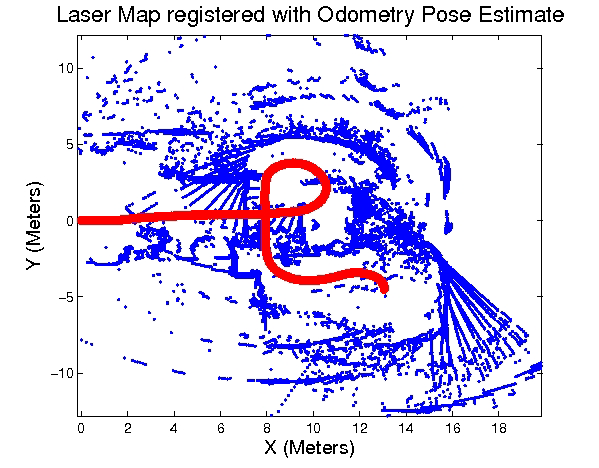
\includegraphics[width=0.4\linewidth]{slam1}
        \hspace{1em}
        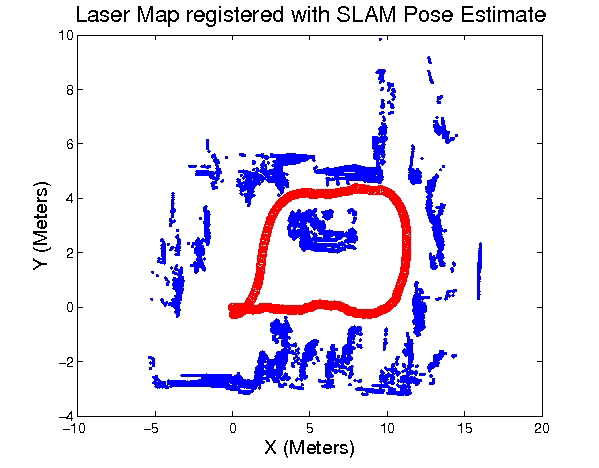
\includegraphics[width=0.4\linewidth]{slam2}
    \end{center}
\end{frame}

\begin{frame}{Example}

\begin{block}{\url{http://youtu.be/Q1ipn42rMh8}}

\end{block}

\end{frame}

\begin{frame}{Commercial applications}

\begin{itemize}
\item \href{https://www.youtube.com/watch?v=bq5HZzGF3vQ}{Samsung vacuum
  cleaning robot}
\item \href{https://www.youtube.com/watch?v=bq5HZzGF3vQ}{iRobot having SLAM}
\end{itemize}

\end{frame}

\section{Path planning on graph}

\begin{frame}{Global path planning}

Assumptions

\begin{itemize}
\item There exists a good enough map of the environment for navigation
  (topological or metric or a mixture between both).
\item The robot knows where it is on the map (using for example GPS or Monte
  Carlo localisation).
\end{itemize}

First step:

\begin{itemize}
\item Representation of the environment by a road-map (graph), cells or a
  potential field. The resulting discrete locations or cells allow then
  to use standard planning algorithms.
\end{itemize}

Examples:

\begin{itemize}
\item Visibility Graph
\item Voronoi Diagram
\item Cell Decomposition -\textgreater{} Connectivity Graph
\item Potential Field
\end{itemize}

\end{frame}

\begin{frame}{Path Planning: Configuration Space}

\begin{itemize}
\item State or configuration $q$ can be described with $k$ values
  $qi$

    \begin{center}
        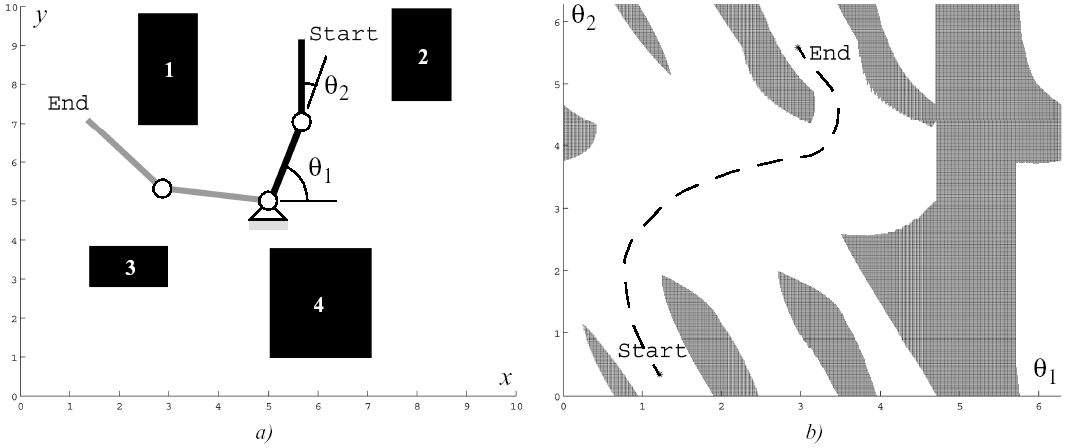
\includegraphics[width=0.6\linewidth]{configurationspace}
    \end{center}

\item \textbf{Configuration space} of a robot: a n-dimensional map of free
  and occupied states.
\end{itemize}

\end{frame}

\begin{frame}{Graphs}

Maps used by robots can be seen as interconnected nodes.

Areas with paths between them are called \textbf{graphs.}

\begin{itemize}
\item \textbf{In maths, the paths are called edges, the areas are called
  nodes.}
\end{itemize}

For example: a visibility graph

    \begin{center}
        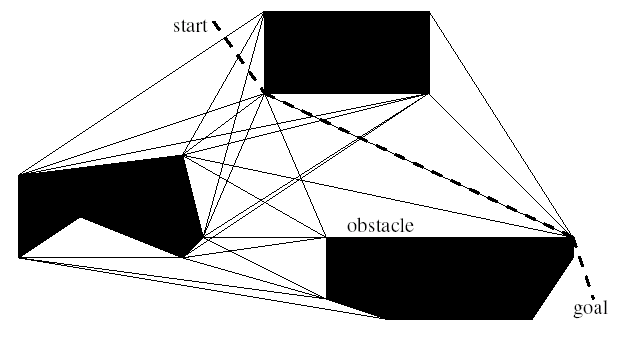
\includegraphics[width=0.6\linewidth]{visibilitygraph}
    \end{center}

Edges between nodes are the lines of sight from each corner to an
obstacle to every other visible corner.

\end{frame}

\begin{frame}{Graphs: Voronoi graphs}

\begin{itemize}
\item Voronoi graph, distance to obstacles from every nodes is maximal.

    \begin{center}
        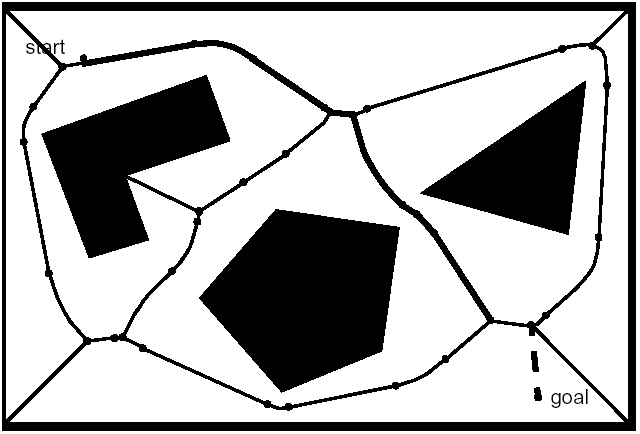
\includegraphics[width=0.8\linewidth]{voronoi}
    \end{center}

\item Works well as the robot's sensors get a get view of the environment.
\end{itemize}

\end{frame}

\begin{frame}{Graphs: Voronoi diagram}

\begin{itemize}
\item SysQuake demo
\end{itemize}

\end{frame}

\begin{frame}{Graphs: Cell Decomposition}

Divide space into simple, connected regions called cells

Determine which open sells are adjacent and construct a connectivity
graph

Find cells in which the initial and goal configuration (state) lie and
search for a path in the connectivity graph to join them.

From the sequence of cells found with an appropriate search algorithm,
compute a path within each cell.

\begin{itemize}
\item e.g. passing through the midpoints of cell boundaries or by sequence
  of wall following movements.
\end{itemize}

\end{frame}

\begin{frame}{Graphs: Cell Decomposition}

Example: exact cell decomposition

    \begin{center}
        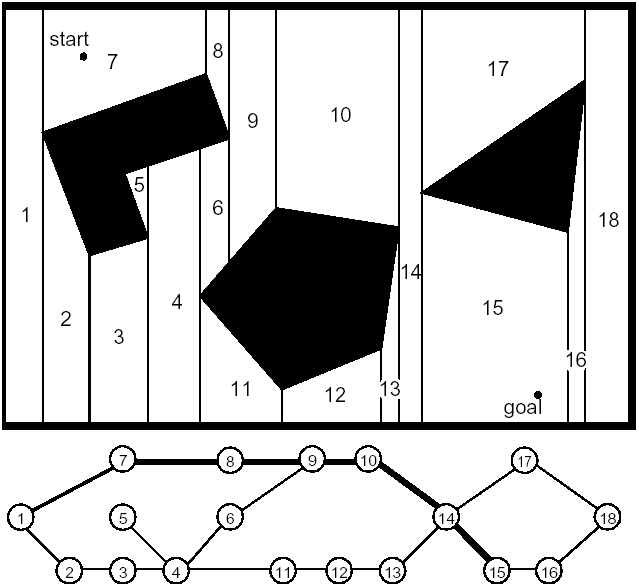
\includegraphics[width=0.8\linewidth]{exactcelldecomposition}
    \end{center}

\end{frame}

\begin{frame}{Graphs: Cell Decomposition}

Example: approximate cell decomposition

    \begin{center}
        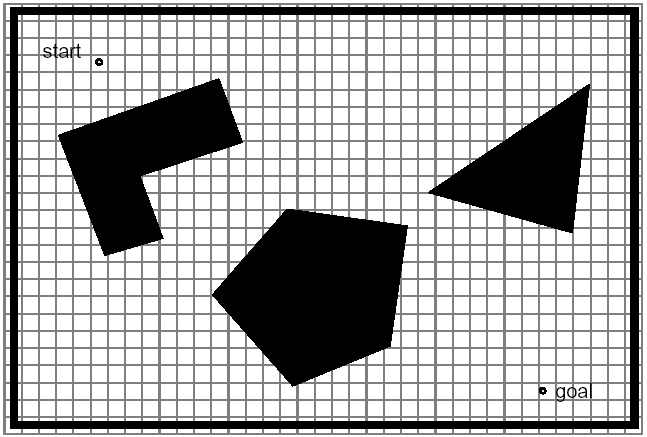
\includegraphics[width=0.4\linewidth]{celldecomposition1}
        \hspace{1em}
        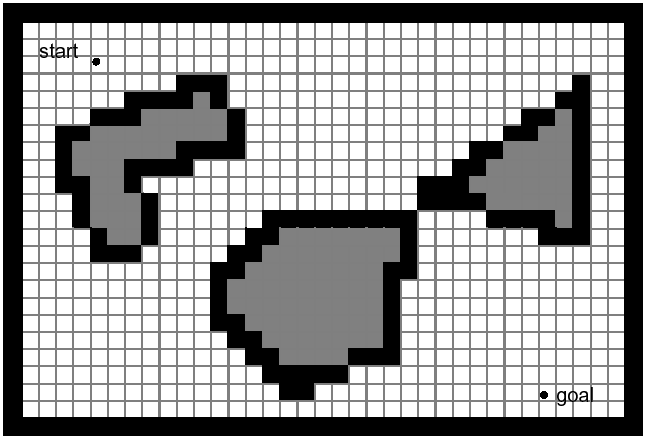
\includegraphics[width=0.4\linewidth]{celldecomposition2}
    \end{center}

\end{frame}

\begin{frame}{Graphs: Cell Decomposition}

Adaptive cell decomposition: changes the size of each cell according
  to the detail needed.

    \begin{center}
        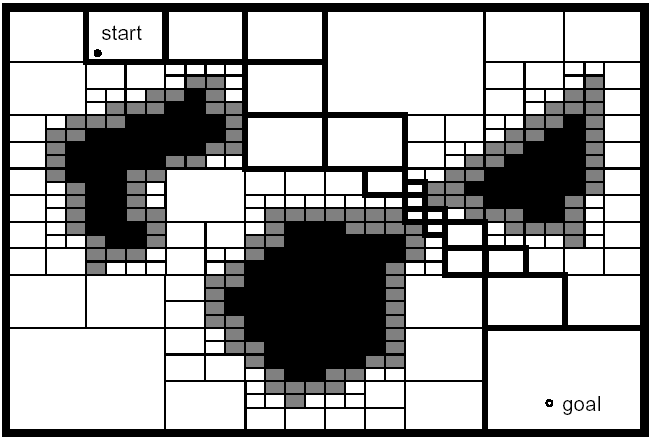
\includegraphics[width=0.8\linewidth]{adaptivecelldecomposition}
    \end{center}
\end{frame}

\begin{frame}{Graphs: representing}

\begin{itemize}
\item How is a graph represented in a computer? Graphical representation is
  intuitive, but not straightforward to implement in a program.
\item Graphs can be represented as a matrix:
\end{itemize}


    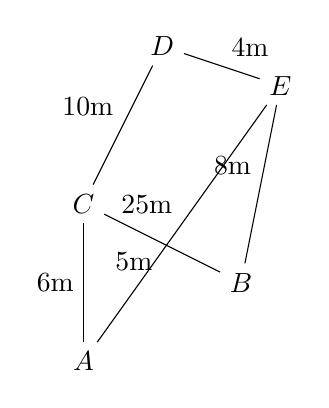
\begin{tikzpicture}[every edge quotes/.style={auto=right}]
        \node at (0,0) (A) {$A$};
        \node at (2,1) (B) {$B$};
        \node at (0,2) (C) {$C$} edge["6m",left] (A)
                                 edge["5m"] (B);
        \node at (1,4) (D) {$D$} edge["10m"] (C);
        \node at (2.5,3.5) (E) {$E$} edge["4m"] (D)
                                     edge["8m"] (B)
                                     edge["25m"] (A);

        %\draw (A) --[label=25m] (E) --[label=4m] (D) --[label=10m] (B) --[label=5m] (C) --[label=6m] (A);
        %\draw (E) --[label=8m] (B);
    \end{tikzpicture}

\end{frame}

\begin{frame}{Searching graphs}

Graphs can be searched, for example to find the shortest path between
two nodes.

Many different search algorithms exist

\begin{itemize}
\item \href{http://en.wikipedia.org/wiki/Breadth-first_search}{Breadth
  first}
\item \href{http://en.wikipedia.org/wiki/Depth-first_search}{Depth first}
\item \href{http://en.wikipedia.org/wiki/A*_search_algorithm}{A*}
\item \href{http://en.wikipedia.org/wiki/Dijkstra's_algorithm}{Dijkstra's
  shortest path}
\end{itemize}

\end{frame}

\begin{frame}[fragile]{Searching graphs - Dijkstra}

\begin{pythoncode}
def dijkstra(graph, weights, start_node):

  dist = {} # map {node -> distance to 'start_node'}
  previous = {} # needed to reconstruct shortest path

  for node in graph:
    dist[node] = math.inf # initial dist. from 'start_node' to 'node'

  dist[start_node] = 0

  Q = graph.nodes() # unvisited nodes
  while not Q.empty():
    u = pop_min(Q) # remove best node

    for v in u.neighbours: # iterate over nodes connected to u
      if dist[u] + weights(u, v) < dist[v]: # new shorter path to v!
        dist[v] = dist[u] + weights(u, v)
        previous[v] = u

  return dist, previous
\end{pythoncode}
\end{frame}


\begin{frame}[fragile]{Searching graphs -- Dijkstra}

Reading out shortest path from the start node to to $t$:

\begin{pythoncode}
path = []
node = t # goal
while node in previous:
    path = [node] + path # append at the front of our path
    node = previous[node]
\end{pythoncode}

Returns the shortest path (if there are more than one, only one is returned).
Return empty if no path exists.

\end{frame}

\begin{frame}{Dijkstra's algorithm: illustration}

    \begin{center}
    \video[1]{0.6\linewidth}{figs/part6/dijkstra.mp4}
    \end{center}

Dijkstra search for finding path between start (red) and goal (green)
position (\href{http://en.wikipedia.org/wiki/Dijkstra's_algorithm}{Wiki
Commons}). Note how Dijkstra is expanding its search out from the
starting position, without knowledge about which nodes could bring it
closer to the goal.

\end{frame}

\begin{frame}{The cost of search}

Maps can be huge

\begin{itemize}
\item For example, 100,000 m2 shopping mall, with a 10x10cm map
  resolution, requires 10 million nodes on the graph.
\end{itemize}

Search time can be problematic

\begin{itemize}
\item Dijkstra has order $O$(N+V2). For example, for a map with 107
  nodes and 108 vertices, it can take 107+102x8 ≈ 1016 calculations to
  find a shortest path between two points.
\item Some implementations are much more efficient. A* search is at worst
  the same as Dijkstra, but can be polynomial in the number of nodes
  $O$(Nk) when a good heuristic is used. For example, if you can
  choose between two nodes to explore, take the node closer to the goal.
\end{itemize}

\end{frame}

\begin{frame}{A* algorithm - illustration}

    \begin{center}
        \video[1]{0.6\linewidth}{figs/part6/astar.mp4}
    \end{center}

A* search for finding path between start and goal position. A* uses a
heuristic (here the distance to the goal
\href{http://en.wikipedia.org/wiki/A*_search_algorithm}{--} it first
expands to nodes closer to the goal) which gives it a chance of finding
the solution in less time.
\href{http://en.wikipedia.org/wiki/A*_search_algorithm}{(Wiki Commons})

\end{frame}

\section{Potential field path planning}

\begin{frame}{Potential Field Path Planning}

Robot is treated as a \emph{point under the influence} of an artificial
potential field.

\begin{itemize}
\item Generated robot movement is similar to a ball rolling down the hill
\item Goal generates attractive force
\item Obstacle are repulsive forces.
\end{itemize}

Needed

\begin{itemize}
\item Location of robot.
\item Location of obstacles.
\item A good way is for these to be on a metric map.
\end{itemize}

\end{frame}

\begin{frame}{Potential Field Path Planning}

    \begin{center}
        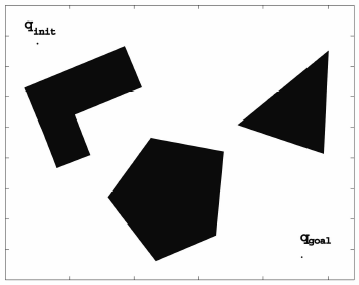
\includegraphics[width=0.4\linewidth]{potentialfields1}

        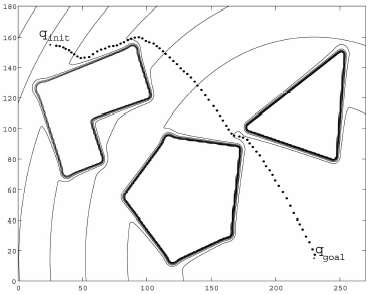
\includegraphics[width=0.4\linewidth]{potentialfields2}
        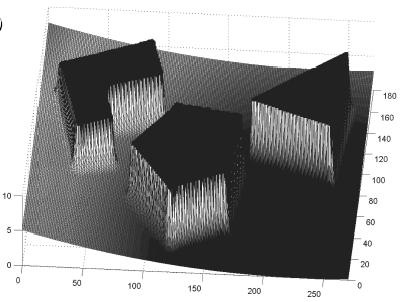
\includegraphics[width=0.4\linewidth]{potentialfields3}
    \end{center}
\end{frame}

\begin{frame}{Potential Field Path Planning}

Potential field generation

Generation of potential field function $U(q)$

\begin{itemize}
\item attracting (goal) and repulsing (obstacle) fields
\item summing up the fields
\item functions must be
  \href{http://en.wikipedia.org/wiki/Differentiable_function}{differentiable}
\end{itemize}

Generate artificial force field $F(q)$

\[
    F(q) = -\nabla U(q) = -\nabla U_{att}(q) - \nabla U_{rep}(q) =
    \begin{bmatrix}\frac{\partial U}{x} \\ \frac{\partial U}{y}\end{bmatrix}
\]

Set robot speed $(v_x, v_y)$ proportional to the force
$F(q)$ generated by the field

\begin{itemize}
\item the force field drives the robot to the goal
\item if robot is assumed to be a point mass
\end{itemize}


\end{frame}

\begin{frame}{Potential Field Path Planning}

Attractive potential field

\begin{itemize}
\item For example, a parabolic function representing the Euclidean distance
  to the goal
\item Attracting force converges linearly towards 0 (goal)
\end{itemize}

\end{frame}

\begin{frame}{Potential Field Path Planning}

Repulsing potential field

Should generate a barrier around all the obstacle

\begin{itemize}
\item strong if close to the obstacle
\item no influence if far from the obstacle
\item Field is positive or zero and \emph{tends to infinity} as q gets
  closer to the object
\end{itemize}

\end{frame}

\begin{frame}{Potential Field Path Planning}

Notes:

\begin{itemize}
\item Local minima problem exists: robot can get stuck in places on the map
  where the potential field has a local dip.
\item problem is getting more complex if the robot is not considered as a
  point mass
\item If objects are convex there exists situations where several minimal
  distances exist ® can result in oscillations
\item Robot path oscillates, e.g. in narrow passages.
\end{itemize}

Sysquake demo

Videos

\begin{itemize}
\item \url{http://www.youtube.com/watch?v=DxzRYYMjxKY}
\item \url{http://www.youtube.com/watch?v=JnPfu7xHNt4}
\end{itemize}

\end{frame}

\begin{frame}{Potential Field Path Planning}

Extended Potential Field Path Planning

Additionally a \emph{rotation potential field} and a \emph{task
potential field} in introduced

Rotation potential field

\begin{itemize}
\item force is also a function of robots orientation to the obstacle
\end{itemize}

Task potential field

\begin{itemize}
\item Filters out the obstacles that should not influence the robots
  movements, i.e. only the obstacles in the sector Z in front of the
  robot are considered
\end{itemize}

\end{frame}

\section{Grassfire algorithm}

\begin{frame}{Grassfire algorithm}

\begin{itemize}
\item Starting from a metric map, a wave front is expanded around the goal.
\item Goal is reaches by travelling on descending values.
\end{itemize}

    \begin{center}
        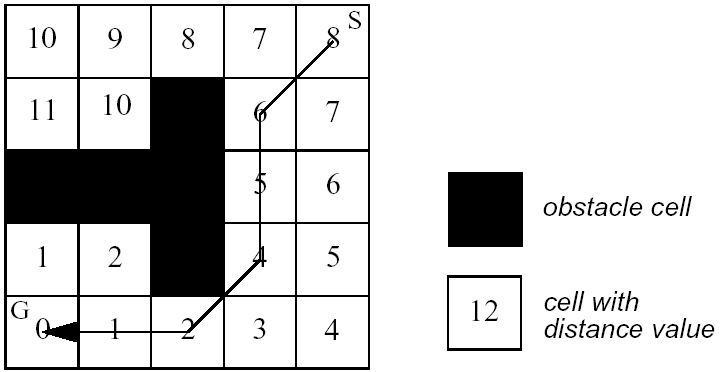
\includegraphics[width=0.6\linewidth]{grassfire}
    \end{center}
\end{frame}

\begin{frame}{Grassfire algorithm}

\end{frame}

\imageframe{grassfire2}

\begin{frame}[fragile]{Grassfire algorithm}

\begin{pythoncode}

def grassfire( M, goal )
  Q = goal # Put goal in queue
  M(goal) := 0 # Set goal value to 0

  while Q is not empty: # Do until map filled
    a := dequeue from Q
    for n := all neighbours of a AND if neighbour no value yet
      if n is not obstacle
        Q := Q enqueue n
        M(n) = M(a) + 1
\end{pythoncode}

Q is a
\href{http://en.wikipedia.org/wiki/Queue_(abstract_data_type)}{queue
data structure}, a first-in first-out list. The queue keeps track of
which locations on the map still need to be visited.

\end{frame}


\begin{frame}{}
    \begin{center}
        \Large
        That's all, folks!\\[2em]
        \normalsize
        Questions:\\
        Portland Square A216 or \url{severin.lemaignan@plymouth.ac.uk} \\[1em]

        Slides:\\ \href{https://github.com/severin-lemaignan/module-mobile-and-humanoid-robots}{\small github.com/severin-lemaignan/module-mobile-and-humanoid-robots}

    \end{center}
\end{frame}



\end{document}
